\section{지금까지의 근거}
\label{sec:evidence}

\begin{figure*}[t]
\centering
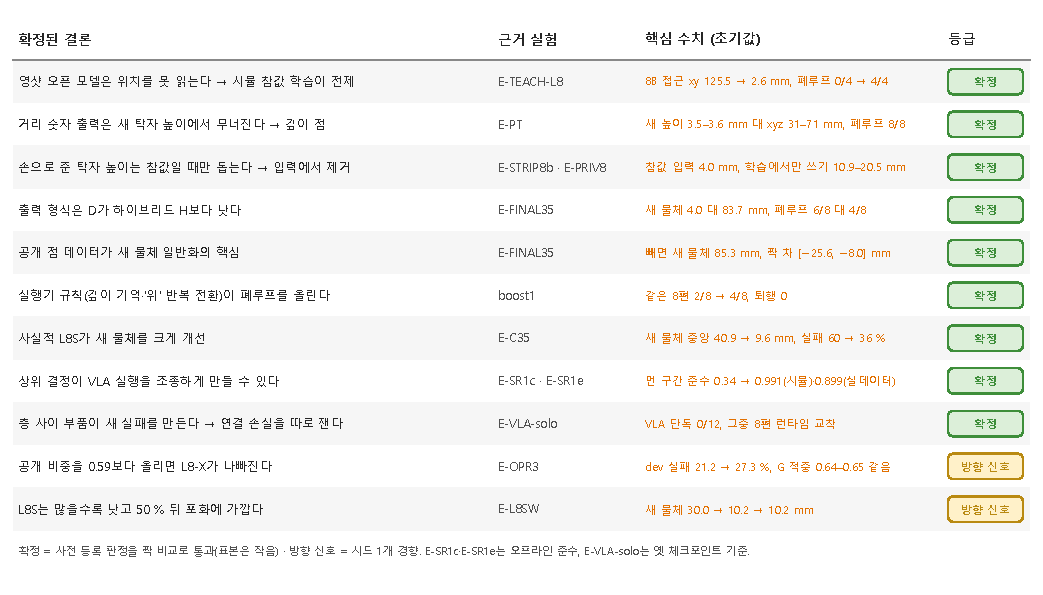
\includegraphics[width=\linewidth]{figures/f8_conclusions.pdf}
\caption{\textbf{확정된 결론 지도.} 결론마다 근거 실험, 핵심 수치(모두 \tentative{초기값}), 신뢰 등급을 적었다. 확정 = 사전 등록 판정을 짝 비교로 통과(표본은 작다). 방향 신호 = 시드 하나의 경향. E-SR1c·E-SR1e는 오프라인 준수이고, E-VLA-solo는 앞선 두 층 구현의 체크포인트 기준이다.}
\label{fig:concl}
\end{figure*}

모든 실험은 판정 규칙을 실행 전에 고정했다. 표본이 작고 시드가 하나인 경우가 많으므로 수치는 모두 초기값이다. \cref{fig:concl}은 지금 확정된 결론을 한눈에 모은 것이다.

\paragraph{상위는 학습해야 조종할 수 있다 (H-L).} 영샷 Qwen3-VL-8B는 접근 목표 xy 오차 중앙이 \tentative{125.5\,mm}였고, 시뮬 참값 라벨로 LoRA 학습하자 \tentative{2.6\,mm}, 폐루프 \tentative{0/4 $\rightarrow$ 4/4}가 되었다(E-TEACH-L8). 영샷 8B에게 점을 찍게 해도 점이 \tentative{55--95\,px} 빗나갔으므로 점 형식도 학습이 전제다.

\paragraph{거리는 깊이 점이 알려 준다.} 같은 편을 출력 형식만 바꿔 비교하자, 깊이 점만 본 적 없는 탁자 높이에서 \tentative{3.5--3.6\,mm}를 유지했고(깊이 없는 xyz \tentative{31--71\,mm}) 폐루프 \tentative{8/8}이었다(E-PT). 참 탁자 높이를 입력한 판만 새 높이에 맞았고(\tentative{4.0\,mm}), 학습에서만 쓰는 세 방법은 \tentative{10.9--20.5\,mm}로 채택 기준을 넘지 못했다(E-STRIP8b, E-PRIV8).

\paragraph{D와 공개 점.} 35B를 D와 하이브리드 H로 학습해 비교하자 새 물체에서 D \tentative{4.0} 대 H \tentative{83.7\,mm}, 폐루프 \tentative{6/8} 대 \tentative{4/8}이었고 나머지 다섯 세트는 같았다(E-FINAL35, 판마다 시드 하나). 공개 점만 뺀 D는 새 물체 \tentative{85.3\,mm}, 폐루프 \tentative{2/8}이었다(짝 차 \tentative{[$-$25.6, $-$8.0]\,mm}). 재학습 없는 실행기 규칙은 같은 8편에서 \tentative{2/8 $\rightarrow$ 4/8}, 퇴행 0이었다(boost1). 이 35B D(f35\_d)가 본 학습의 비교 기준이다.


\paragraph{데이터 구성.} 사실적 L8S로 만든 확인판(E-C35)은 새 물체 OOD-O58 오차 중앙을 \tentative{40.9 $\rightarrow$ 9.6\,mm}, 실패율을 \tentative{60 $\rightarrow$ 36\,\%}로 줄였다. 반면 L8-X dev 실패(\tentative{16.8 $\rightarrow$ 27.5\,\%})와 OOD-H(\tentative{17.3 $\rightarrow$ 22.8\,\%})는 나빠졌다. 공개 비중을 0.59보다 올리면 L8-X가 나빠지고 G는 나아지지 않았다(E-OPR3, \cref{fig:evidence}c). L8S는 많을수록 나았고 50\,\% 뒤로는 포화에 가까웠다(E-L8SW, \cref{fig:evidence}b). 두 결과 모두 시드 하나의 방향 신호다.

\paragraph{본 35B.} 1 에폭에서 새 물체 오차 중앙·실패율은 \tentative{9.5\,mm / 34.8\,\%}로 f35\_d(\tentative{40.9\,mm / 60\,\%})보다 크게 나았다. L8-X dev \tentative{4.5\,mm / 18.9\,\%}(f35\_d \tentative{4.4 / 16.8}), OOD-H \tentative{4.0 / 17.3}(같음), OOD-O \tentative{4.1 / 37.4}(\tentative{4.1 / 40.8}), 일반 평가 G 적중 \tentative{0.742}(\tentative{0.713}), L8S 보류 \tentative{5.5\,mm / 23.7\,\%}였다. 확인판에서 벌어졌던 옛 도메인 차이는 학습이 진행될수록 줄어(\cref{fig:evidence}d), 그 손해가 도메인보다 양 때문이라는 해석과 맞는다. 최종 판정은 사전 등록한 최적 에폭에서 낸다.

\paragraph{결합 쪽 근거.} 상위 결정 토큰만 바꿔서는 VLA의 행동 청크가 거의 움직이지 않았다(강제 방향 준수 \tentative{0.34}, 우연 약 0.33, E-SR0). 물체에서 먼 구간의 반사실 분기를 흐름 정합 학습에 섞자 준수가 시뮬 \tentative{0.991}(E-SR1c), 실데이터 \tentative{0.899}(E-SR1e, 두 시드)로 올랐고 접촉 근처 능력은 비열등이었다. 오프라인 준수이며 폐루프 확인은 아니다. 앞선 두 층 구현에서 VLA 단독은 모든 조건에서 \tentative{0/12}였고(같은 장면 스크립트 기준선 \tentative{12/12}), 그중 \tentative{8}편은 모델이 아니라 층 사이 런타임의 멈춤 고리였다(E-VLA-solo). 층 사이의 부품이 새 실패를 만든다는 이 결과가, 연결 손실을 따로 재는 이유다.

\paragraph{JCR를 따로 학습해야 한다 (E-CJ1).} 상위 없이 시뮬 참값 명령을 주고, 같은 시드(머그$\rightarrow$쟁반, 20 배치 $\times$ 기본·무작위화 = 팔당 40편)에서 세 팔을 비교했다. 스크립트 실행기(OX)는 \tentative{40/40}, 앞의 오프라인 준수 \tentative{0.991} 체크포인트를 조이스틱으로 쓴 OV는 \tentative{1/40}, 같은 모델의 단독 모드(V0)는 \tentative{0/40}이었다. 등록 규칙상 이 모델은 조이스틱으로도 과제를 못 하는 바닥(VLA\_FLOOR)이므로 2$\times$2보다 JCR 학습이 먼저다. OV의 결정 스텝 약 10,000개를 나눠 보면 원인은 네 가지다.
\begin{itemize}
  \item \textbf{분포 이동:} 폐루프 xy 준수는 \tentative{0.41}(목표에서 먼 구간 \tentative{0.47})로, 학습 분포 안 상태에서 잰 오프라인 \tentative{0.991}과 달랐다. 좌표계 오류의 흔적(일정한 회전)은 없었다.
  \item \textbf{근접 구간을 배운 적 없음:} 반사실 분기가 먼 구간에만 있었다. 목표 2\,cm 안 스텝의 \tentative{77\,\%}가 오히려 멀어졌고(준수 \tentative{0.33}), 손은 대상 위 3--9\,cm에서 맴돌았다.
  \item \textbf{거친 조이스틱:} 8방향·5단 크기·축별 1\,cm 사각지대라 방향 양자화 오차가 90분위 \tentative{35$^\circ$}였고, 8\,mm 수렴이 구조적으로 어려웠다.
  \item \textbf{청크 이음 계단:} 청크 첫 행과 현재 관절의 차가 중앙 \tentative{0.065\,rad}로, 청크의 \tentative{87.5\,\%}가 0.04\,rad 한도에 잘렸다. 또 그리퍼 시점은 접촉이 아니라 단계 문장을 따랐다.
\end{itemize}
지연은 원인이 아니었다(모델 호출 동안 시뮬 시간이 멈춤). 네 원인이 JCR 설계의 네 선택, 곧 자기 롤아웃 재라벨, 근접 분기, 연속 조이스틱, 명령 기준 TCP 변위 청크와 단계 문장 제거로 이어진다(\cref{sec:vla}).
